% Created 2017-03-18 Sat 05:14
% Intended LaTeX compiler: pdflatex
\documentclass[bigger]{beamer}
\usepackage[utf8]{inputenc}
\usepackage[T1]{fontenc}
\usepackage{fixltx2e}
\usepackage{graphicx}
\usepackage{longtable}
\usepackage{float}
\usepackage{wrapfig}
\usepackage{rotating}
\usepackage[normalem]{ulem}
\usepackage{amsmath}
\usepackage{textcomp}
\usepackage{marvosym}
\usepackage{wasysym}
\usepackage{amssymb}
\usepackage{hyperref}
\tolerance=1000
\usepackage{minted}
\usepackage{mycmds}
\usepackage{pgfplots}
\usepackage[german, germanb]{babel}
\uselanguage{german}
\usepackage{url}
\usepackage{pgfplots}
\usetikzlibrary{pgfplots.groupplots}
\pdfmapfile{+sansmathaccent.map}
\mode<beamer>{\usetheme{Berkeley}}
\usetheme{default}
\author{Stephan Messlinger, Valentin Ochs}
\date{\today}
\title{Blinkenlights Workshop}
\hypersetup{
 pdfauthor={Stephan Messlinger, Valentin Ochs},
 pdftitle={Blinkenlights Workshop},
 pdfkeywords={},
 pdfsubject={},
 pdfcreator={Emacs 25.2.1 (Org mode 9.0.5)}, 
 pdflang={Germanb}}
\begin{document}

\maketitle

\section{Digital Out}
\label{sec:org365a622}
\begin{frame}[fragile,label={sec:org8c67f30}]{Startpunkt digitaler Output}
 Blink Beispiel: File \(\rightarrow\) Examples \(\rightarrow\) Basics \(\rightarrow\) Blink

\begin{minted}[]{c}
void setup() {
  pinMode(13, OUTPUT);
}

void loop() {
  digitalWrite(13, HIGH);
  delay(1000);
  digitalWrite(13, LOW);
  delay(1000);
}
\end{minted}
\end{frame}

\begin{frame}[fragile,label={sec:org73facc3}]{Setup}
 \texttt{pinMode(pin, modus)} wählt für den Pin mit Nummer \texttt{pin} eine von drei
Betriebsarten:

\begin{itemize}
\item \texttt{OUTPUT}: wird für Ausgabe verwendet, z.B. um LEDs zu schalten oder
mit anderen Microcontrollern zu sprechen.
\item \texttt{INPUT}: Die Spannung am Pin kann gelesen werden.
\item \texttt{INPUT\_PULLUP}: Wie \texttt{INPUT}, aber der Pin wird intern auf die
Versorgunsspannung gezogen.
\end{itemize}
\end{frame}

\begin{frame}[fragile,label={sec:org7e2609f}]{digitalWrite und delay}
 \texttt{digitalWrite(pin, zustand)} setzt bei einem auf Output gestellten Pin
die Ausgangsspannung:

\begin{itemize}
\item 0 Volt für \texttt{LOW}
\item 5 Volt für \texttt{HIGH} (oder was auch immer die aktuelle
Versorgungsspannung ist)
\end{itemize}

\texttt{delay(ms)} tut \texttt{ms} Millisekunden lang nichts.
\end{frame}

\begin{frame}[fragile,label={sec:org86d78a0}]{Andere Blink Muster}
 Zwei Sekunden lang an, eine halbe aus.

\pause

\begin{minted}[]{c}
digitalWrite(13, HIGH);
delay(2000);
digitalWrite(13, LOW);
delay(500);
\end{minted}
\end{frame}

\begin{frame}[label={sec:orgaa27ad5}]{Schnelleres Blinken}
Was passiert, wenn man die Zeiten ganz niedrig setzt?
\pause

\(\rightarrow\) Man sieht kein Blinken mehr
\pause

Was passiert, wenn die Zeitverhältnisse geändert werden?
\pause

\(\rightarrow\) Dimmen
\end{frame}

\section{Analog Out}
\label{sec:orga26fa18}
\begin{frame}[fragile,label={sec:org6dd008e}]{analogWrite}
 \texttt{analogWrite(pin, wert)} schaltet den Pin automatisch an und aus, mit
variablen An-/Aus-Zeiten 

\(\rightarrow\) Pulsweitenmodulation

\begin{itemize}
\item Frequenz: Etwa 490 Hz
\item Wertebereich: 0 bis 255
\item Nur auf Pins 3, 5, 6, 9, 10, und 11.
\item Die PWM Pins sind auf dem Arduino mit \textasciitilde{} markiert.
\end{itemize}
\end{frame}

\begin{frame}[label={sec:orgac95e39}]{PWM Funktionsweise: Zähler + Vergleich}
\begin{LATEX}
\begin{tikzpicture}
\begin{axis}[xlabel=Zeit / s, ylabel=Zähler, ymin=-0.02*256, ymax=1.02*256]
\addplot[blue, domain=0:0.001, samples=512] { floor(mod(x*490*2*pi*256, 256)) };
\addplot[red, domain=0:0.001, samples=2] { 128 };
\end{axis}
\end{tikzpicture}
\end{LATEX}
\end{frame}

\begin{frame}[label={sec:org5b0b1ba}]{PWM, Schwellwert 128}
\begin{LATEX}
\begin{tikzpicture}
\begin{axis}[xlabel=Zeit / s, ylabel=Spannung / V, ymin=-0.1, ymax=5.1]
\addplot[blue, domain=0:0.001, samples=500] { 5*ceil(0.5-mod(x*490*2*pi, 1)) };
\addplot[red, domain=0:0.001, samples=2] { 2.5 };
\end{axis}
\end{tikzpicture}
\end{LATEX}
\end{frame}

\begin{frame}[label={sec:orgad18e5d}]{PWM, Schwellwert 16}
\begin{LATEX}
\begin{tikzpicture}
\begin{axis}[xlabel=Zeit / s, ylabel=Spannung / V, ymin=-0.1, ymax=5.1]
\addplot[blue, domain=0:0.001, samples=500] { 5*ceil(0.0625-mod(x*490*2*pi, 1)) };
\addplot[red, domain=0:0.001, samples=2] { 16./256 };
\end{axis}
\end{tikzpicture}
\end{LATEX}
\end{frame}

\begin{frame}[fragile,label={sec:org64089f9}]{Einfacher PWM Code}
 \begin{minted}[]{c}
void setup() {
  pinMode(11, OUTPUT);
}
void loop() {
  // Zeit seit Beginn des Programms
  unsigned long time = millis();
  // Berechne eine Sägezahn mit 0.1 Hz
  int value = 255 * time / 4000;
  // Verwende den Wert als Schwellwert
  analogWrite(11, value);
}
\end{minted}
\end{frame}

\begin{frame}[label={sec:org902231c}]{PWM Frequenz}
490 Hz sind bei schnellen Bewegungen sichtbar.

Bestimmung der Frequenz: Taktfrequenz / Vorteiler / Zählergrö\ss{}e

\begin{itemize}
\item Taktfrequenz: 16 MHz
\item Zählergrö\ss{}e:
\begin{itemize}
\item 256 für Pins 5 und 6
\item 510 für 3, 9, 10, 11
\end{itemize}
\end{itemize}
\end{frame}

\begin{frame}[fragile,label={sec:org232a711}]{PWM Vorteiler: Timer 0, Pins 5 und 6}
 \begin{center}
\begin{tabular}{rrr}
Einstellung & Teiler & Frequenz\\
\hline
0x01 & 1 & 62500\\
0x02 & 8 & 7813\\
0x03 & 64 & 977\\
0x04 & 256 & 244\\
0x05 & 1024 & 61\\
\end{tabular}
\end{center}

Einstellen durch
\begin{minted}[]{c}
TCCR0B = (TCCR0B & 0b11111000) | Einstellung
\end{minted}
\end{frame}

\begin{frame}[fragile,label={sec:orgf37ded2}]{PWM Vorteiler: Timer 1, Pins 9 und 10}
 \begin{center}
\begin{tabular}{rrr}
Einstellung & Teiler & Frequenz\\
\hline
0x01 & 1 & 31373\\
0x02 & 8 & 3921\\
0x03 & 64 & 490\\
0x04 & 256 & 123\\
0x05 & 1024 & 31\\
\end{tabular}
\end{center}

Einstellen durch
\begin{minted}[]{c}
TCCR1B = (TCCR0B & 0b11111000) | Einstellung
\end{minted}
\end{frame}

\begin{frame}[fragile,label={sec:org4ab3286}]{PWM Vorteiler: Timer 2, Pins 11 und 3}
 \begin{center}
\begin{tabular}{rrr}
Einstellung & Teiler & Frequenz\\
\hline
0x01 & 1 & 31373\\
0x02 & 8 & 3921\\
0x03 & 32 & 980\\
0x04 & 64 & 490\\
0x05 & 128 & 245\\
0x06 & 256 & 123\\
0x07 & 1024 & 31\\
\end{tabular}
\end{center}

Einstellen durch
\begin{minted}[]{c}
TCCR2B = (TCCR2B & 0b11111000) | Einstellung
\end{minted}
\end{frame}

\begin{frame}[fragile,label={sec:orgfbf39f2}]{Vorsicht}
 Frequenzänderung beeinflusst nicht nur LEDs, sondern alles, was an dem
Timer hängt! Servos, Tonerzeugung, etc.

Besonders wichtig: Timer 0 für \texttt{millis()} und
\texttt{delay()}. Standardvorteiler: 64. Bei Änderungen Zeiten entsprechend
anpassen (Vervierfachen bei 256\ldots{})
\end{frame}

\section{Digital In}
\label{sec:orgdf1ee2f}
\begin{frame}[label={sec:org9b6e7ef}]{Startpunkt digitaler Input}
Button Beispiel: File \(\rightarrow\) Examples \(\rightarrow\) Digital
\(\rightarrow\) Button

Geht nicht nur mit einfachen Schaltern und Tastern, sondern auch
z.B. einer Lichtschranke oder Reed-Schaltern.
\end{frame}

\begin{frame}[fragile,label={sec:org88c87b9}]{digitalRead}
 \texttt{digitalRead(pin)}: 
\begin{itemize}
\item \texttt{HIGH} falls Spannung an \texttt{pin} etwa 2.6 V oder höher
\item \texttt{LOW} falls Spannung an \texttt{pin} 2.1 V oder tiefer
\item Nur bei 5 V Versorgungsspannung, sonst andere Werte
\end{itemize}
\end{frame}

\begin{frame}[label={sec:orgd099c4e}]{Schaltplanvarianten}
\begin{center}
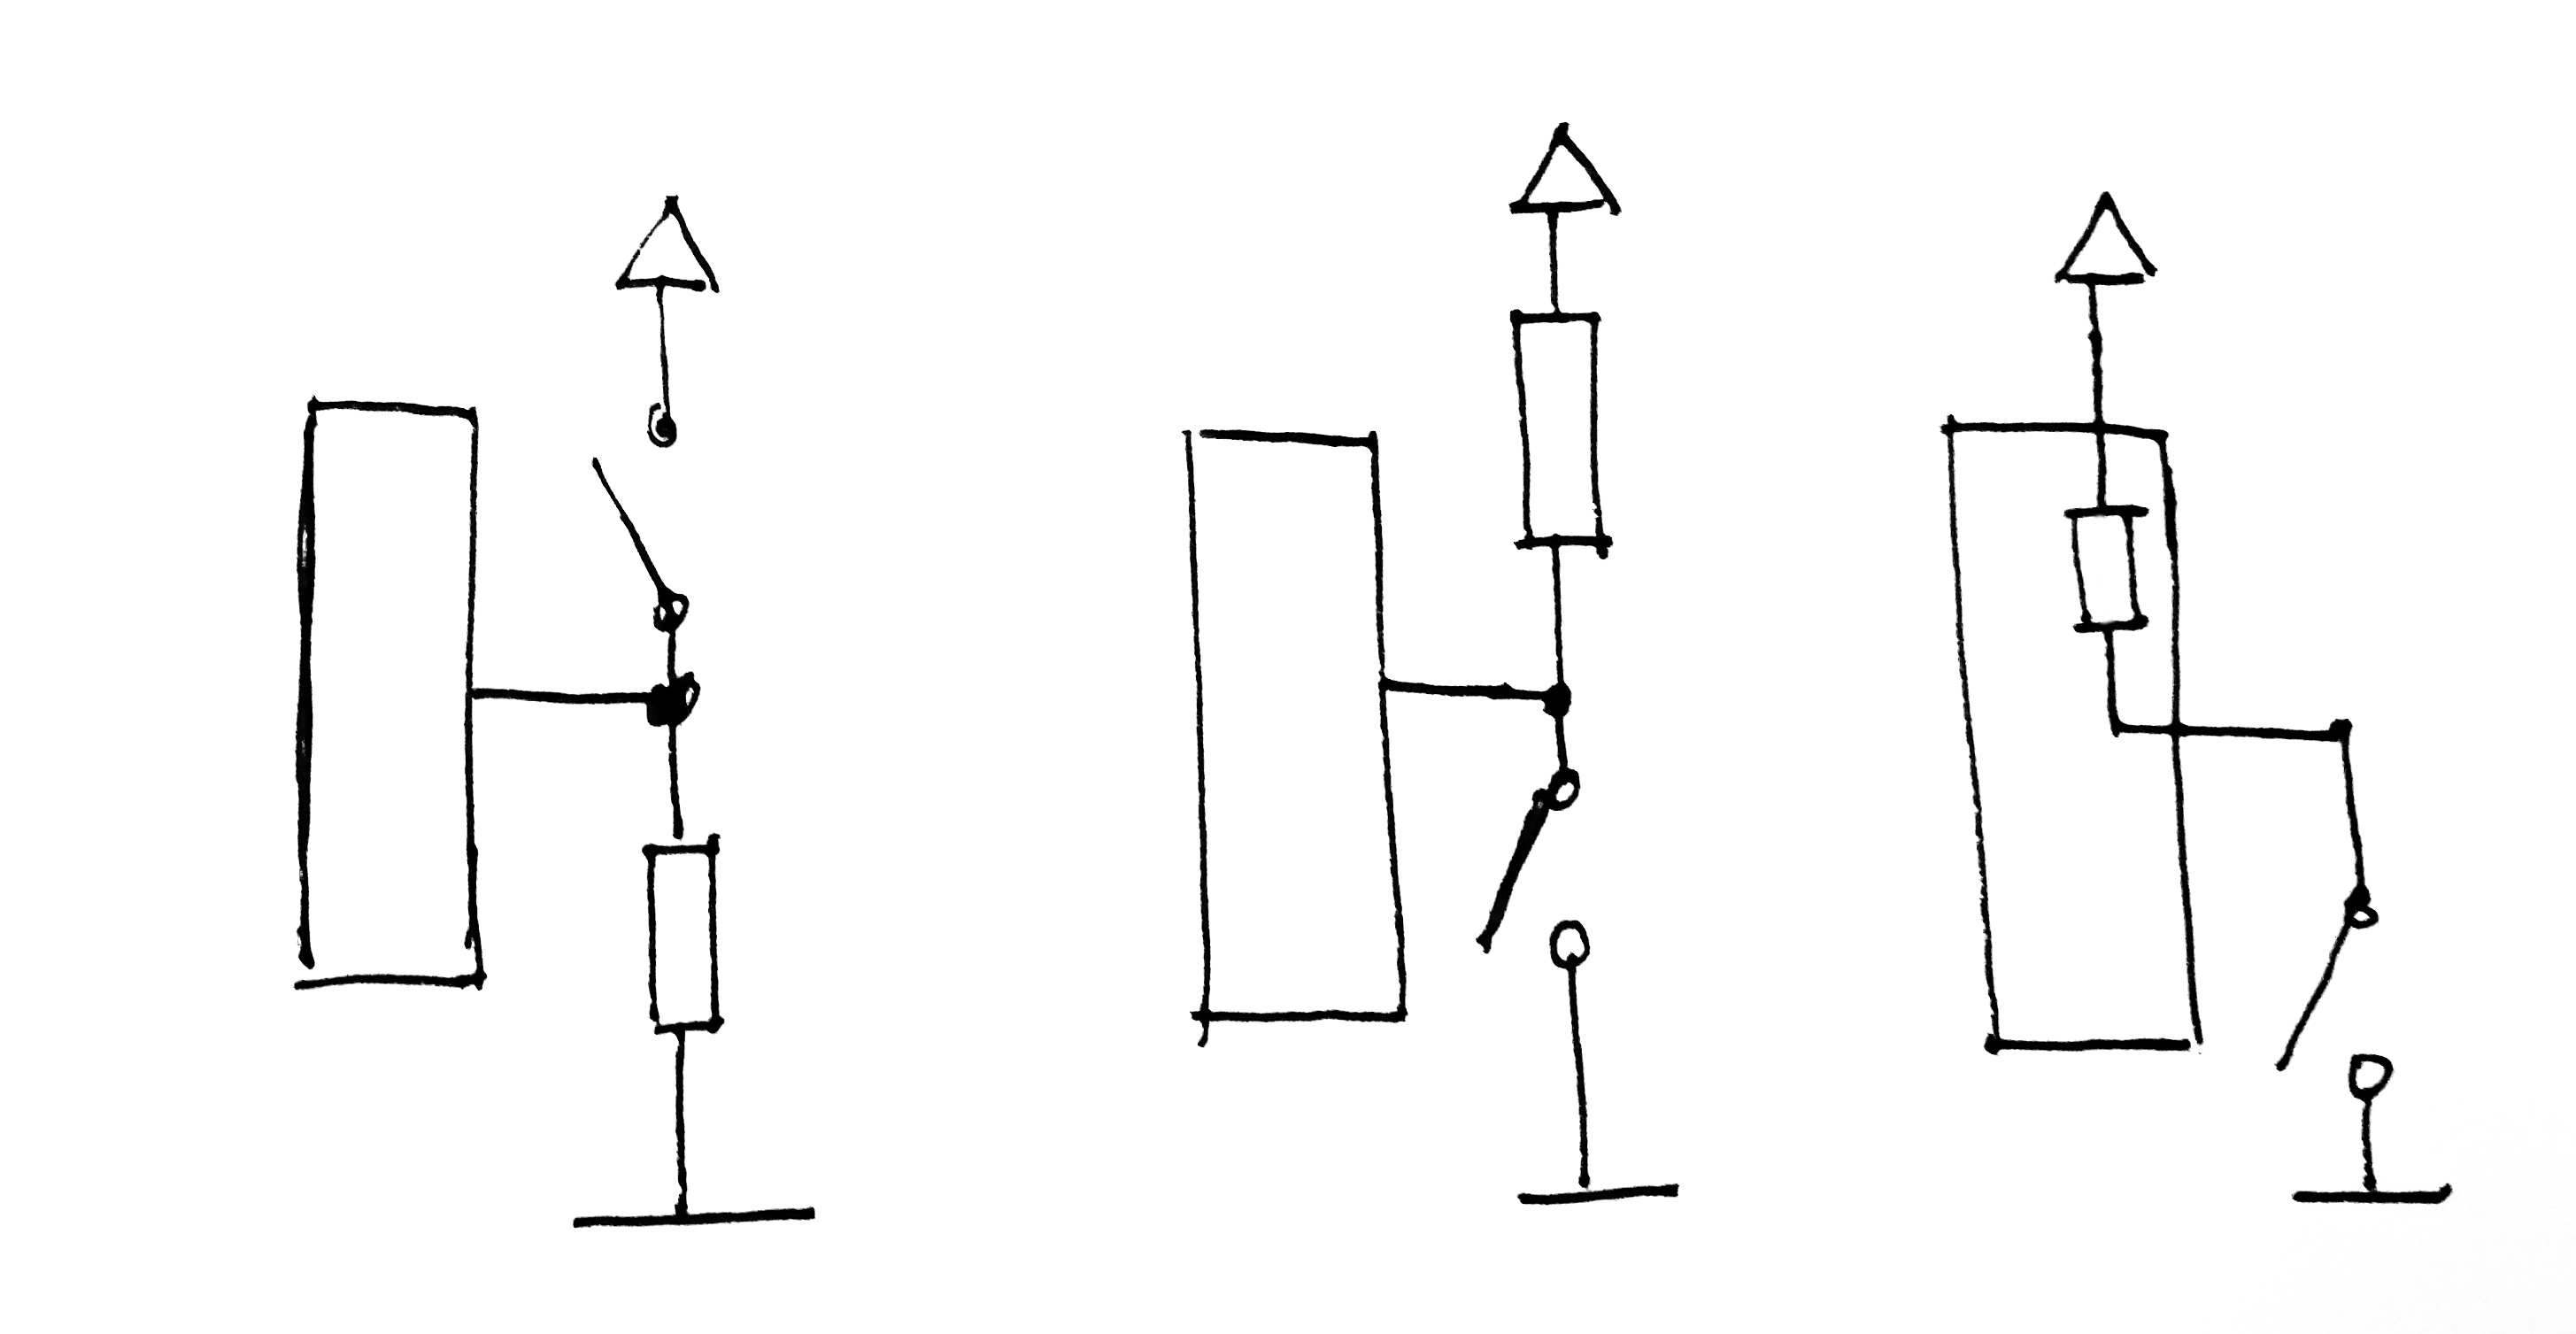
\includegraphics[width=.9\linewidth]{./img/pullup.jpg}
\end{center}
\end{frame}

\begin{frame}[fragile,label={sec:org2585c8e}]{Unterbrechbare Abläufe starten (1)}
 \begin{minted}[]{c}
unsigned long button_time = 0;
bool running = false;
void loop() {
  if(digitalRead(button_pin) == HIGH) {
    running = true;
    button_time = millis();
  }
  if(running) {
    running = do_stuff(millis() - start_time);
  }
}
\end{minted}
\end{frame}

\begin{frame}[fragile,label={sec:org295e77e}]{Unterbrechbare Abläufe starten (2)}
 \begin{minted}[]{c}
bool do_stuff(unsigned long time_point)
  if(time_point < 100) {
    digitalWrite(led_pin, HIGH);
  } else if(time_point < 200) {
    digitalWrite(led_pin, LOW);
  } else if(time_point < 1000) {
    digitalWrite(led_pin, HIGH);
  } else {
    return false;
  }
  return true;
}
\end{minted}
\end{frame}

\begin{frame}[label={sec:org005125d}]{Prellen}
\begin{center}
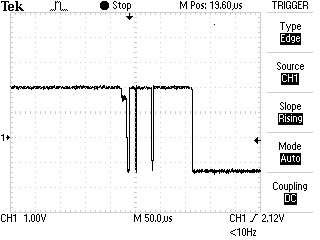
\includegraphics[width=.9\linewidth]{./img/bounce.png}
\end{center}
\end{frame}

\begin{frame}[label={sec:org4dc2daf}]{Entprellen}
Auch: Debouncing

\begin{itemize}
\item Hardware Lösung: Tiefpassfilter mit Kondensator
\item Software Lösung: Mehrmals Wert auslesen und warten, bis er sich
nicht mehr ändert
\item Hier ohne weitere Vertiefung, aber ihr wisst jetzt, wonach man
suchen muss :)
\end{itemize}
\end{frame}

\section{Analog In}
\label{sec:org10e6fbc}
\begin{frame}[label={sec:orgf5b0d44}]{Startpunkt analoger Input}
AnalogInput Beispiel: File \(\rightarrow\) Examples \(\rightarrow\) Analog
\(\rightarrow\) AnalogInput
\end{frame}

\begin{frame}[fragile,label={sec:org8a58234}]{analogRead}
 \texttt{analogRead(pin)}: 0-1023 für 0-5 Volt an Pin \texttt{pin}.
\end{frame}

\begin{frame}[fragile,label={sec:org4750e9b}]{Kombination mit analogWrite}
 \begin{minted}[]{c}
void loop() {
  int value = analogRead(A0) / 4;
  analogWrite(3, value);
}
\end{minted}
\end{frame}
\end{document}
